\documentclass{article}
\usepackage{amsmath} 
\usepackage{amssymb} 
\usepackage{pgfplots}
\usepackage{fancyhdr}


\pagestyle{fancy}
\fancyhf{}
\rhead{\thepage} % Page number on the right side
\lhead{\textit{Domain, Range, Graph of Function | Rafi Ahmed Saad }} 
\renewcommand{\headrulewidth}{0.5pt}

\title{Function Exercises}
\author{Rafi Ahmed Saad}
\date{\today}

\begin{document}
\maketitle % This generates the title based on \title, \author, and \date

\section{Functions}
\subsection{Find the domain and range of $f(x) = \frac{x^2 - 1}{x-1}$}

Domain is all possible inputes for which the function is defined. In this case,
we need to avoid values of $x$ that makes the denominator equal to zero, as
division by zero is undefined. Thus the domain is all real numbers except $x =
	1$, because that would make the denominator $x - 1 = 0$

\[ \text{Domain: } x \in \mathbb{R} \setminus \{1\} \]

\paragraph{Let function}
\begin{align*}
	f(x)             & = \frac{(x^2 - 1)}{x - 1}      \\
	\Rightarrow f(x) & = \frac{(x - 1)(x + 1)}{x - 1} \\
	\Rightarrow f(x) & = x + 1                        \\
	\therefore \text{Range: } f(x) \in \mathbb{R}
\end{align*}

\begin{tikzpicture}
	\begin{axis}[
			axis lines = center,
			xlabel = $x$,
			ylabel = $f(x)$,
			domain = -5:5,
			samples = 100,
			legend pos = north west,
		]
		\addplot[blue, mark=none] {(x^2 - 1)/(x - 1)} node[pos=0.8, below right] {$\frac{(x^2 - 1)}{x - 1} $};
		\legend{$f(x) = \frac{x^2 - 1}{x - 1}$}
	\end{axis}
\end{tikzpicture}

\newpage
\subsection{Find the domain and range of \[
		f(x) = \begin{cases}
			2x + 6 & \text{if } -3 \leq x \leq 0 \\
			6      & \text{if } 0 \le x \le 2    \\
			2x - 6 & \text{if } 2 \leq x \leq 5
		\end{cases}
	\]}

\subsection*{Domain: }
The domain of $f(x)$ is set to all possible inputes values for which the
function is defined. In this case, the function is defined in the intervals
$[-3, 0], [0, 2], [2, 5]$, and for any other values, it is not explicitly
defind. So the domain is:

\[ \text{Domain: } x \in [-3, 0] \cup [0, 2] \cup [2, 5] \]
\[  x \in [-3, 5] \]

\subsection*{Range: }
For $ -3 \leq x \leq 0 \text{, } f(x) = 2x + 6 $ where the output varies from 0
to 6\\ For $ 0 \leq x \leq 2 \text{, } f(x) = 6 $\\ For $ 2 \leq x \leq 5
	\text{, } f(x) = 2x - 6 $ where the ouptu varies from -2 to 4 \\ So the Range
is:
\[
	\text{Ragne: } f(x) \in [0, 6] \cup [-2, 4] \\
	\rightarrow f(x) \in [-2, 6]
\]

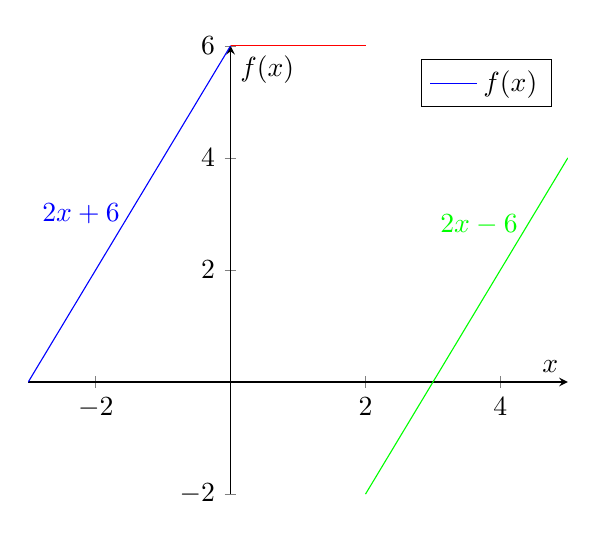
\begin{tikzpicture}
	\begin{axis}[
			axis lines = center,
			xlabel = $x$,
			ylabel = $f(x)$,
			domain = -3:5,
			samples = 1000,
			legend pos = north east,
		]
		\addplot[blue, domain=-3:0] {2*x + 6} node[pos=0.5, left] {$2x + 6$};
		\addplot[red, domain=0:2] {6} node[pos=0.5, above] {6};
		\addplot[green, domain=2:5] {2*x - 6} node[pos=0.8, left] {$2x - 6$};
		\legend{$f(x)$}
	\end{axis}
\end{tikzpicture}

\newpage
\subsection{Find the domain and range of \[
		f(x) = \begin{cases}
			x - 1 & \text{if } x > 0 \\ - \frac{1}{2} & \text{if } x = 0 \\ x + 1 &
			   \text{if } x < 0
		\end{cases}
	\]}

\subsection*{Domain: }
Domain of this function $f(x)$ can take any input.
\begin{align*}
	\therefore \text{Domain: } & x \in \mathbb{R}\\
	\text{Domain: } & x \in (-\infty, \infty)
\end{align*}

\subsection*{Range: }
For $x > 0$, $f(x) = x - 1$ where the result of the function is $[0, \infty]$
\\ \\ For $x = 0$, $f(x) = -\frac{1}{2}$ which is a constant value \\ \\ For
${x < 0}$, $f(x) = x + 1$ where the result of the function is $[0, -\infty]$

\begin{align*}
	\therefore \text{Range: } & x \in [0, -\infty] \cup [\frac{1}{2}] \cup [0, \infty] \\
	\text{Range: }            & x \in (-\infty, \infty)
\end{align*}
\\
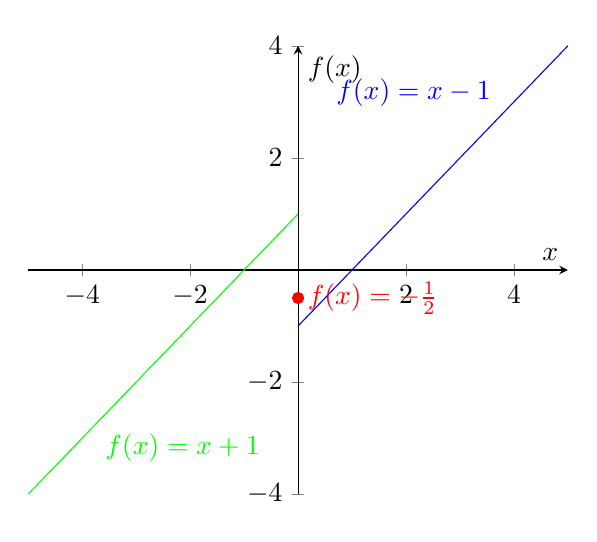
\begin{tikzpicture}
	\begin{axis}[
			axis lines = center,
			xlabel = $x$,
			ylabel = $f(x)$,
			domain = -5:5,
			samples = 100,
			legend pos = north east,
		]
		\addplot[blue, domain=0:5] {x - 1} node[pos=0.75, above left] {$f(x) = x - 1$};
		\addplot[red, mark=*] coordinates {(0, -1/2)} node[pos=0.5, right] {$f(x) = -\frac{1}{2}$};
		\addplot[green, domain=-5:0] {x + 1} node[pos=0.25, below right] {$f(x) = x + 1$};
	\end{axis}
\end{tikzpicture}

\newpage
\subsection{Find the domain and range of \[
	f(x) = \begin{cases}
		-2x + 1 	& \text{if } x < 0 \\ 
		1			& \text{if } 0 \leq x < 1\\ 
		2x - 1 		& \text{if } x \geq 1
	\end{cases}
	\]}

\subsection*{Domain: }
Domain of this function $f(x)$ can take any input.
\begin{align*}
	\therefore \text{Domain: } & x \in \mathbb{R}\\
	\text{Domain: } & x \in (-\infty, \infty)
\end{align*}

\subsection*{Range: }
For $x < 0 \text{, } f(x) = -2x + 1$ where the result of the function is $(-\infty, 1]$
\\ \\
For $0 \leq x < 1$, $f(x) = 1$ which is a constant value \\ \\ 
For ${x \geq 1}$, $f(x) = 2x - 1$ where the result of the function is $[1, \infty)$

\begin{align*}
	\therefore \text{Range: } & x \in (-\infty, 1] \cup [1] \cup [1, \infty) \\
	\text{Range: }            & x \in (-\infty, \infty)
\end{align*}
\\
\begin{tikzpicture}
    \begin{axis}[
        axis lines = center,
        xlabel = $x$,
        ylabel = $f(x)$,
        domain = -10:10, % Adjust the domain according to your needs
        samples = 100,
        legend pos = north east,
    ]
        \addplot[blue, domain=-10:0] {-2*x + 1} node[pos=0.5, above right] {$-2x + 1$};
        \addplot[red, domain=0:1] {1} node[pos=0.5, above] {$1$};
        \addplot[green, domain=1:10] {2*x - 1} node[pos=0.25, below right] {$2x - 1$};
    \end{axis}
\end{tikzpicture}

\newpage
\subsection{Find the domain and range of \[
	f(x) = \begin{cases}
		x 		& \text{if } 0 \leq x < \frac{1}{2} \\ 
		1		& \text{if } x = \frac{1}{2}\\ 
		1-x 	& \text{if } \frac{1}{2} < x \leq 1
	\end{cases}
	\]}

\subsection*{Domain: }
The domain of the function $f(x)$ is all possible input values for which the function is defined. In this case, the intervals are $[0, \frac{1}{2}) \text{, } [\frac{1}{2}] \text{, } (\frac{1}{2}, 1]$. So the domain is:
\begin{align*}
	\text{Domain: } & x \in [0, \frac{1}{2}) \cup [\frac{1}{2}] \cup (\frac{1}{2}, 1]\\
	\text{Domain: } & x \in [0, 1]
\end{align*}

\subsection*{Range: }
For $0 \leq x < \frac{1}{2} \text{, } f(x) = x$ where the result of the function is $[0, \frac{1}{2})$
\\ \\
For $ x = \frac{1}{2}$, $f(x) = 1$ which is a constant value. So the range is [1]\\ \\ 
For $\frac{1}{2} < x \leq 1$, $f(x) = 1 - x$ where the result of the function is $[\frac{1}{2}, 1]$

\begin{align*}
	\therefore \text{Range: } & x \in [0, \frac{1}{2}) \cup \left\{ 1 \right\} \cup (\frac{1}{2}, 1] \\
	\text{Range: }            & x \in [0, \frac{1}{2}) \cup \left\{ 1 \right\}
\end{align*}
\\
\begin{tikzpicture}
    \begin{axis}[
        axis lines = center,
        xlabel = $x$,
        ylabel = $f(x)$,
        domain = 0:1, % Adjust the domain according to your needs
        samples = 100,
        legend pos = north east,
    ]
        \addplot[blue, domain=0:0.5] {x} node[pos=0.75, above left] {$x$};
        \addplot[red, mark=*] coordinates {(0.5, 1)} node[pos=0.8, right] {$1$};
        \addplot[green, domain=0.5:1] {1-x} node[pos=0.5, right] {$1-x$};
    \end{axis}
\end{tikzpicture}


\end{document}
